\documentclass[1p]{elsarticle_modified}
%\bibliographystyle{elsarticle-num}

%\usepackage[colorlinks]{hyperref}
%\usepackage{abbrmath_seonhwa} %\Abb, \Ascr, \Acal ,\Abf, \Afrak
\usepackage{amsfonts}
\usepackage{amssymb}
\usepackage{amsmath}
\usepackage{amsthm}
\usepackage{scalefnt}
\usepackage{amsbsy}
\usepackage{kotex}
\usepackage{caption}
\usepackage{subfig}
\usepackage{color}
\usepackage{graphicx}
\usepackage{xcolor} %% white, black, red, green, blue, cyan, magenta, yellow
\usepackage{float}
\usepackage{setspace}
\usepackage{hyperref}

\usepackage{tikz}
\usetikzlibrary{arrows}

\usepackage{multirow}
\usepackage{array} % fixed length table
\usepackage{hhline}

%%%%%%%%%%%%%%%%%%%%%
\makeatletter
\renewcommand*\env@matrix[1][\arraystretch]{%
	\edef\arraystretch{#1}%
	\hskip -\arraycolsep
	\let\@ifnextchar\new@ifnextchar
	\array{*\c@MaxMatrixCols c}}
\makeatother %https://tex.stackexchange.com/questions/14071/how-can-i-increase-the-line-spacing-in-a-matrix
%%%%%%%%%%%%%%%

\usepackage[normalem]{ulem}

\newcommand{\msout}[1]{\ifmmode\text{\sout{\ensuremath{#1}}}\else\sout{#1}\fi}
%SOURCE: \msout is \stkout macro in https://tex.stackexchange.com/questions/20609/strikeout-in-math-mode

\newcommand{\cancel}[1]{
	\ifmmode
	{\color{red}\msout{#1}}
	\else
	{\color{red}\sout{#1}}
	\fi
}

\newcommand{\add}[1]{
	{\color{blue}\uwave{#1}}
}

\newcommand{\replace}[2]{
	\ifmmode
	{\color{red}\msout{#1}}{\color{blue}\uwave{#2}}
	\else
	{\color{red}\sout{#1}}{\color{blue}\uwave{#2}}
	\fi
}

\newcommand{\Sol}{\mathcal{S}} %segment
\newcommand{\D}{D} %diagram
\newcommand{\A}{\mathcal{A}} %arc


%%%%%%%%%%%%%%%%%%%%%%%%%%%%%5 test

\def\sl{\operatorname{\textup{SL}}(2,\Cbb)}
\def\psl{\operatorname{\textup{PSL}}(2,\Cbb)}
\def\quan{\mkern 1mu \triangleright \mkern 1mu}

\theoremstyle{definition}
\newtheorem{thm}{Theorem}[section]
\newtheorem{prop}[thm]{Proposition}
\newtheorem{lem}[thm]{Lemma}
\newtheorem{ques}[thm]{Question}
\newtheorem{cor}[thm]{Corollary}
\newtheorem{defn}[thm]{Definition}
\newtheorem{exam}[thm]{Example}
\newtheorem{rmk}[thm]{Remark}
\newtheorem{alg}[thm]{Algorithm}

\newcommand{\I}{\sqrt{-1}}
\begin{document}

%\begin{frontmatter}
%
%\title{Boundary parabolic representations of knots up to 8 crossings}
%
%%% Group authors per affiliation:
%\author{Yunhi Cho} 
%\address{Department of Mathematics, University of Seoul, Seoul, Korea}
%\ead{yhcho@uos.ac.kr}
%
%
%\author{Seonhwa Kim} %\fnref{s_kim}}
%\address{Center for Geometry and Physics, Institute for Basic Science, Pohang, 37673, Korea}
%\ead{ryeona17@ibs.re.kr}
%
%\author{Hyuk Kim}
%\address{Department of Mathematical Sciences, Seoul National University, Seoul 08826, Korea}
%\ead{hyukkim@snu.ac.kr}
%
%\author{Seokbeom Yoon}
%\address{Department of Mathematical Sciences, Seoul National University, Seoul, 08826,  Korea}
%\ead{sbyoon15@snu.ac.kr}
%
%\begin{abstract}
%We find all boundary parabolic representation of knots up to 8 crossings.
%
%\end{abstract}
%\begin{keyword}
%    \MSC[2010] 57M25 
%\end{keyword}
%
%\end{frontmatter}

%\linenumbers
%\tableofcontents
%
\newcommand\colored[1]{\textcolor{white}{\rule[-0.35ex]{0.8em}{1.4ex}}\kern-0.8em\color{red} #1}%
%\newcommand\colored[1]{\textcolor{white}{ #1}\kern-2.17ex	\textcolor{white}{ #1}\kern-1.81ex	\textcolor{white}{ #1}\kern-2.15ex\color{red}#1	}

{\Large $\underline{11a_{90}~(K11a_{90})}$}

\setlength{\tabcolsep}{10pt}
\renewcommand{\arraystretch}{1.6}
\vspace{1cm}\begin{tabular}{m{100pt}>{\centering\arraybackslash}m{274pt}}
\multirow{5}{120pt}{
	\centering
	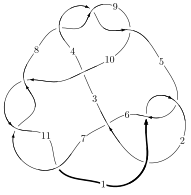
\includegraphics[width=112pt]{../../../GIT/diagram.site/Diagrams/png/339_11a_90.png}\\
\ \ \ A knot diagram\footnotemark}&
\allowdisplaybreaks
\textbf{Linearized knot diagam} \\
\cline{2-2}
 &
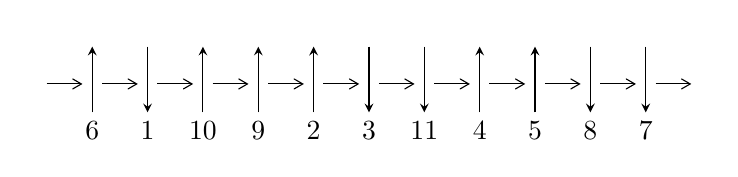
\begin{tikzpicture}[x=20pt, y=17pt]
	% nodes
	\node (C0) at (0, 0) {};
	\node (C1) at (1, 0) {};
	\node (C1U) at (1, +1) {};
	\node (C1D) at (1, -1) {6};

	\node (C2) at (2, 0) {};
	\node (C2U) at (2, +1) {};
	\node (C2D) at (2, -1) {1};

	\node (C3) at (3, 0) {};
	\node (C3U) at (3, +1) {};
	\node (C3D) at (3, -1) {10};

	\node (C4) at (4, 0) {};
	\node (C4U) at (4, +1) {};
	\node (C4D) at (4, -1) {9};

	\node (C5) at (5, 0) {};
	\node (C5U) at (5, +1) {};
	\node (C5D) at (5, -1) {2};

	\node (C6) at (6, 0) {};
	\node (C6U) at (6, +1) {};
	\node (C6D) at (6, -1) {3};

	\node (C7) at (7, 0) {};
	\node (C7U) at (7, +1) {};
	\node (C7D) at (7, -1) {11};

	\node (C8) at (8, 0) {};
	\node (C8U) at (8, +1) {};
	\node (C8D) at (8, -1) {4};

	\node (C9) at (9, 0) {};
	\node (C9U) at (9, +1) {};
	\node (C9D) at (9, -1) {5};

	\node (C10) at (10, 0) {};
	\node (C10U) at (10, +1) {};
	\node (C10D) at (10, -1) {8};

	\node (C11) at (11, 0) {};
	\node (C11U) at (11, +1) {};
	\node (C11D) at (11, -1) {7};
	\node (C12) at (12, 0) {};

	% arrows
	\draw[->,>={angle 60}]
	(C0) edge (C1) (C1) edge (C2) (C2) edge (C3) (C3) edge (C4) (C4) edge (C5) (C5) edge (C6) (C6) edge (C7) (C7) edge (C8) (C8) edge (C9) (C9) edge (C10) (C10) edge (C11) (C11) edge (C12) ;	\draw[->,>=stealth]
	(C1D) edge (C1U) (C2U) edge (C2D) (C3D) edge (C3U) (C4D) edge (C4U) (C5D) edge (C5U) (C6U) edge (C6D) (C7U) edge (C7D) (C8D) edge (C8U) (C9D) edge (C9U) (C10U) edge (C10D) (C11U) edge (C11D) ;
	\end{tikzpicture} \\
\hhline{~~} \\& 
\textbf{Solving Sequence} \\ \cline{2-2} 
 &
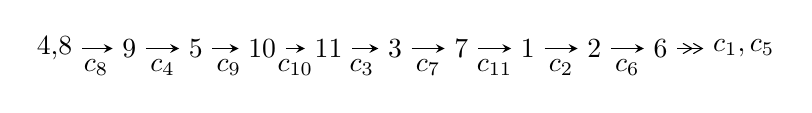
\begin{tikzpicture}[x=24pt, y=7pt]
	% node
	\node (A0) at (-1/8, 0) {4,8};
	\node (A1) at (1, 0) {9};
	\node (A2) at (2, 0) {5};
	\node (A3) at (3, 0) {10};
	\node (A4) at (4, 0) {11};
	\node (A5) at (5, 0) {3};
	\node (A6) at (6, 0) {7};
	\node (A7) at (7, 0) {1};
	\node (A8) at (8, 0) {2};
	\node (A9) at (9, 0) {6};
	\node (C1) at (1/2, -1) {$c_{8}$};
	\node (C2) at (3/2, -1) {$c_{4}$};
	\node (C3) at (5/2, -1) {$c_{9}$};
	\node (C4) at (7/2, -1) {$c_{10}$};
	\node (C5) at (9/2, -1) {$c_{3}$};
	\node (C6) at (11/2, -1) {$c_{7}$};
	\node (C7) at (13/2, -1) {$c_{11}$};
	\node (C8) at (15/2, -1) {$c_{2}$};
	\node (C9) at (17/2, -1) {$c_{6}$};
	\node (A10) at (41/4, 0) {$c_{1},c_{5}$};

	% edge
	\draw[->,>=stealth]	
	(A0) edge (A1) (A1) edge (A2) (A2) edge (A3) (A3) edge (A4) (A4) edge (A5) (A5) edge (A6) (A6) edge (A7) (A7) edge (A8) (A8) edge (A9) ;
	\draw[->>,>={angle 60}]	
	(A9) edge (A10);
\end{tikzpicture} \\ 

\end{tabular} \\

\footnotetext{
The image of knot diagram is generated by the software ``\textbf{Draw programme}" developed by Andrew Bartholomew(\url{http://www.layer8.co.uk/maths/draw/index.htm\#Running-draw}), where we modified some parts for our purpose(\url{https://github.com/CATsTAILs/LinksPainter}).
}\phantom \\ \newline 
\centering \textbf{Ideals for irreducible components\footnotemark of $X_{\text{par}}$} 
 
\begin{align*}
I^u_{1}&=\langle 
u^{43}- u^{42}+\cdots+u^2+1\rangle \\
\\
\end{align*}
\raggedright * 1 irreducible components of $\dim_{\mathbb{C}}=0$, with total 43 representations.\\
\footnotetext{All coefficients of polynomials are rational numbers. But the coefficients are sometimes approximated in decimal forms when there is not enough margin.}
\newpage
\renewcommand{\arraystretch}{1}
\centering \section*{I. $I^u_{1}= \langle u^{43}- u^{42}+\cdots+u^2+1 \rangle$}
\flushleft \textbf{(i) Arc colorings}\\
\begin{tabular}{m{7pt} m{180pt} m{7pt} m{180pt} }
\flushright $a_{4}=$&$\begin{pmatrix}0\\u\end{pmatrix}$ \\
\flushright $a_{8}=$&$\begin{pmatrix}1\\0\end{pmatrix}$ \\
\flushright $a_{9}=$&$\begin{pmatrix}1\\- u^2\end{pmatrix}$ \\
\flushright $a_{5}=$&$\begin{pmatrix}u\\- u^3+u\end{pmatrix}$ \\
\flushright $a_{10}=$&$\begin{pmatrix}- u^2+1\\u^4-2 u^2\end{pmatrix}$ \\
\flushright $a_{11}=$&$\begin{pmatrix}- u^4+u^2+1\\u^4-2 u^2\end{pmatrix}$ \\
\flushright $a_{3}=$&$\begin{pmatrix}- u^5+2 u^3- u\\u^7-3 u^5+2 u^3+u\end{pmatrix}$ \\
\flushright $a_{7}=$&$\begin{pmatrix}u^8-3 u^6+u^4+2 u^2+1\\- u^8+4 u^6-4 u^4\end{pmatrix}$ \\
\flushright $a_{1}=$&$\begin{pmatrix}- u^{12}+5 u^{10}-7 u^8+2 u^4+3 u^2+1\\u^{12}-6 u^{10}+12 u^8-8 u^6+u^4-2 u^2\end{pmatrix}$ \\
\flushright $a_{2}=$&$\begin{pmatrix}u^{31}-14 u^{29}+\cdots+20 u^5+8 u^3\\- u^{31}+15 u^{29}+\cdots-8 u^5+u\end{pmatrix}$ \\
\flushright $a_{6}=$&$\begin{pmatrix}u^{20}-9 u^{18}+\cdots+3 u^2+1\\- u^{22}+10 u^{20}+\cdots-10 u^4- u^2\end{pmatrix}$\\ \flushright $a_{6}=$&$\begin{pmatrix}u^{20}-9 u^{18}+\cdots+3 u^2+1\\- u^{22}+10 u^{20}+\cdots-10 u^4- u^2\end{pmatrix}$\\&\end{tabular}
\flushleft \textbf{(ii) Obstruction class $= -1$}\\~\\
\flushleft \textbf{(iii) Cusp Shapes $= -4 u^{41}+80 u^{39}+\cdots+8 u+2$}\\~\\
\newpage\renewcommand{\arraystretch}{1}
\flushleft \textbf{(iv) u-Polynomials at the component}\newline \\
\begin{tabular}{m{50pt}|m{274pt}}
Crossings & \hspace{64pt}u-Polynomials at each crossing \\
\hline $$\begin{aligned}c_{1},c_{5}\end{aligned}$$&$\begin{aligned}
&u^{43}- u^{42}+\cdots+2 u-1
\end{aligned}$\\
\hline $$\begin{aligned}c_{2}\end{aligned}$$&$\begin{aligned}
&u^{43}+19 u^{42}+\cdots-2 u-1
\end{aligned}$\\
\hline $$\begin{aligned}c_{3}\end{aligned}$$&$\begin{aligned}
&u^{43}-3 u^{42}+\cdots-165 u+88
\end{aligned}$\\
\hline $$\begin{aligned}c_{4},c_{8},c_{9}\end{aligned}$$&$\begin{aligned}
&u^{43}+u^{42}+\cdots- u^2-1
\end{aligned}$\\
\hline $$\begin{aligned}c_{6}\end{aligned}$$&$\begin{aligned}
&u^{43}+u^{42}+\cdots-3 u-2
\end{aligned}$\\
\hline $$\begin{aligned}c_{7},c_{10},c_{11}\end{aligned}$$&$\begin{aligned}
&u^{43}-5 u^{42}+\cdots+52 u-7
\end{aligned}$\\
\hline
\end{tabular}\\~\\
\newpage\renewcommand{\arraystretch}{1}
\flushleft \textbf{(v) Riley Polynomials at the component}\newline \\
\begin{tabular}{m{50pt}|m{274pt}}
Crossings & \hspace{64pt}Riley Polynomials at each crossing \\
\hline $$\begin{aligned}c_{1},c_{5}\end{aligned}$$&$\begin{aligned}
&y^{43}+19 y^{42}+\cdots-2 y-1
\end{aligned}$\\
\hline $$\begin{aligned}c_{2}\end{aligned}$$&$\begin{aligned}
&y^{43}+11 y^{42}+\cdots-10 y-1
\end{aligned}$\\
\hline $$\begin{aligned}c_{3}\end{aligned}$$&$\begin{aligned}
&y^{43}-21 y^{42}+\cdots+171017 y-7744
\end{aligned}$\\
\hline $$\begin{aligned}c_{4},c_{8},c_{9}\end{aligned}$$&$\begin{aligned}
&y^{43}-41 y^{42}+\cdots-2 y-1
\end{aligned}$\\
\hline $$\begin{aligned}c_{6}\end{aligned}$$&$\begin{aligned}
&y^{43}+3 y^{42}+\cdots-163 y-4
\end{aligned}$\\
\hline $$\begin{aligned}c_{7},c_{10},c_{11}\end{aligned}$$&$\begin{aligned}
&y^{43}+47 y^{42}+\cdots-1090 y-49
\end{aligned}$\\
\hline
\end{tabular}\\~\\
\newpage\flushleft \textbf{(vi) Complex Volumes and Cusp Shapes}
$$\begin{array}{c|c|c}  
\text{Solutions to }I^u_{1}& \I (\text{vol} + \sqrt{-1}CS) & \text{Cusp shape}\\
 \hline 
\begin{aligned}
u &= -0.450941 + 0.686624 I\end{aligned}
 & \phantom{-}5.35054 - 9.10731 I & \phantom{-}3.33084 + 7.84073 I \\ \hline\begin{aligned}
u &= -0.450941 - 0.686624 I\end{aligned}
 & \phantom{-}5.35054 + 9.10731 I & \phantom{-}3.33084 - 7.84073 I \\ \hline\begin{aligned}
u &= \phantom{-}0.463007 + 0.675614 I\end{aligned}
 & \phantom{-}7.17544 + 3.78029 I & \phantom{-}6.09678 - 3.29694 I \\ \hline\begin{aligned}
u &= \phantom{-}0.463007 - 0.675614 I\end{aligned}
 & \phantom{-}7.17544 - 3.78029 I & \phantom{-}6.09678 + 3.29694 I \\ \hline\begin{aligned}
u &= -0.512233 + 0.637578 I\end{aligned}
 & \phantom{-}5.58121 + 4.70276 I & \phantom{-}4.01683 - 1.90768 I \\ \hline\begin{aligned}
u &= -0.512233 - 0.637578 I\end{aligned}
 & \phantom{-}5.58121 - 4.70276 I & \phantom{-}4.01683 + 1.90768 I \\ \hline\begin{aligned}
u &= \phantom{-}1.180680 + 0.070474 I\end{aligned}
 & -0.12031 + 3.39708 I & -1.05977 - 4.64882 I \\ \hline\begin{aligned}
u &= \phantom{-}1.180680 - 0.070474 I\end{aligned}
 & -0.12031 - 3.39708 I & -1.05977 + 4.64882 I \\ \hline\begin{aligned}
u &= \phantom{-}0.496416 + 0.648800 I\end{aligned}
 & \phantom{-}7.30167 + 0.61667 I & \phantom{-}6.46762 - 2.84316 I \\ \hline\begin{aligned}
u &= \phantom{-}0.496416 - 0.648800 I\end{aligned}
 & \phantom{-}7.30167 - 0.61667 I & \phantom{-}6.46762 + 2.84316 I \\ \hline\begin{aligned}
u &= -0.447772 + 0.632332 I\end{aligned}
 & \phantom{-}1.69784 - 2.06717 I & \phantom{-}0.16713 + 3.29698 I \\ \hline\begin{aligned}
u &= -0.447772 - 0.632332 I\end{aligned}
 & \phantom{-}1.69784 + 2.06717 I & \phantom{-}0.16713 - 3.29698 I \\ \hline\begin{aligned}
u &= -1.25034\phantom{ +0.000000I}\end{aligned}
 & \phantom{-}2.53757\phantom{ +0.000000I} & \phantom{-}3.48810\phantom{ +0.000000I} \\ \hline\begin{aligned}
u &= -1.304990 + 0.171072 I\end{aligned}
 & \phantom{-}1.15199 - 1.78064 I & \phantom{-0.000000 } 0 \\ \hline\begin{aligned}
u &= -1.304990 - 0.171072 I\end{aligned}
 & \phantom{-}1.15199 + 1.78064 I & \phantom{-0.000000 } 0 \\ \hline\begin{aligned}
u &= \phantom{-}0.206694 + 0.605749 I\end{aligned}
 & -2.00685 + 5.68843 I & -2.34470 - 8.72951 I \\ \hline\begin{aligned}
u &= \phantom{-}0.206694 - 0.605749 I\end{aligned}
 & -2.00685 - 5.68843 I & -2.34470 + 8.72951 I \\ \hline\begin{aligned}
u &= -1.356100 + 0.215927 I\end{aligned}
 & \phantom{-}2.91900 - 8.67200 I & \phantom{-0.000000 } 0 \\ \hline\begin{aligned}
u &= -1.356100 - 0.215927 I\end{aligned}
 & \phantom{-}2.91900 + 8.67200 I & \phantom{-0.000000 } 0 \\ \hline\begin{aligned}
u &= \phantom{-}1.366840 + 0.185574 I\end{aligned}
 & \phantom{-}5.03487 + 4.10356 I & \phantom{-0.000000 } 0 \\ \hline\begin{aligned}
u &= \phantom{-}1.366840 - 0.185574 I\end{aligned}
 & \phantom{-}5.03487 - 4.10356 I & \phantom{-0.000000 } 0 \\ \hline\begin{aligned}
u &= \phantom{-}1.403260 + 0.118432 I\end{aligned}
 & \phantom{-}6.22218 + 2.77486 I & \phantom{-0.000000 } 0 \\ \hline\begin{aligned}
u &= \phantom{-}1.403260 - 0.118432 I\end{aligned}
 & \phantom{-}6.22218 - 2.77486 I & \phantom{-0.000000 } 0 \\ \hline\begin{aligned}
u &= -1.411730 + 0.074872 I\end{aligned}
 & \phantom{-}5.35002 + 1.81991 I & \phantom{-0.000000 } 0 \\ \hline\begin{aligned}
u &= -1.411730 - 0.074872 I\end{aligned}
 & \phantom{-}5.35002 - 1.81991 I & \phantom{-0.000000 } 0 \\ \hline\begin{aligned}
u &= \phantom{-}0.089033 + 0.575299 I\end{aligned}
 & -3.14805 - 0.90482 I & -6.51420 - 0.21846 I \\ \hline\begin{aligned}
u &= \phantom{-}0.089033 - 0.575299 I\end{aligned}
 & -3.14805 + 0.90482 I & -6.51420 + 0.21846 I \\ \hline\begin{aligned}
u &= -0.221219 + 0.523394 I\end{aligned}
 & \phantom{-}0.01425 - 1.49737 I & \phantom{-}1.74832 + 5.31506 I \\ \hline\begin{aligned}
u &= -0.221219 - 0.523394 I\end{aligned}
 & \phantom{-}0.01425 + 1.49737 I & \phantom{-}1.74832 - 5.31506 I \\ \hline\begin{aligned}
u &= \phantom{-}0.504381 + 0.191157 I\end{aligned}
 & -0.50303 - 2.82096 I & \phantom{-}3.24990 + 2.85228 I\\
 \hline 
 \end{array}$$\newpage$$\begin{array}{c|c|c}  
\text{Solutions to }I^u_{1}& \I (\text{vol} + \sqrt{-1}CS) & \text{Cusp shape}\\
 \hline 
\begin{aligned}
u &= \phantom{-}0.504381 - 0.191157 I\end{aligned}
 & -0.50303 + 2.82096 I & \phantom{-}3.24990 - 2.85228 I \\ \hline\begin{aligned}
u &= \phantom{-}1.47320 + 0.22968 I\end{aligned}
 & \phantom{-}7.89812 + 5.22510 I & \phantom{-0.000000 } 0 \\ \hline\begin{aligned}
u &= \phantom{-}1.47320 - 0.22968 I\end{aligned}
 & \phantom{-}7.89812 - 5.22510 I & \phantom{-0.000000 } 0 \\ \hline\begin{aligned}
u &= -0.353298 + 0.351162 I\end{aligned}
 & \phantom{-}0.686131 - 1.038760 I & \phantom{-}5.50415 + 5.16099 I \\ \hline\begin{aligned}
u &= -0.353298 - 0.351162 I\end{aligned}
 & \phantom{-}0.686131 + 1.038760 I & \phantom{-}5.50415 - 5.16099 I \\ \hline\begin{aligned}
u &= \phantom{-}1.48315 + 0.24777 I\end{aligned}
 & \phantom{-}11.6071 + 12.5188 I & \phantom{-0.000000 } 0 \\ \hline\begin{aligned}
u &= \phantom{-}1.48315 - 0.24777 I\end{aligned}
 & \phantom{-}11.6071 - 12.5188 I & \phantom{-0.000000 } 0 \\ \hline\begin{aligned}
u &= -1.48567 + 0.24134 I\end{aligned}
 & \phantom{-}13.4835 - 7.1271 I & \phantom{-0.000000 } 0 \\ \hline\begin{aligned}
u &= -1.48567 - 0.24134 I\end{aligned}
 & \phantom{-}13.4835 + 7.1271 I & \phantom{-0.000000 } 0 \\ \hline\begin{aligned}
u &= -1.49208 + 0.22410 I\end{aligned}
 & \phantom{-}13.7502 - 3.7932 I & \phantom{-0.000000 } 0 \\ \hline\begin{aligned}
u &= -1.49208 - 0.22410 I\end{aligned}
 & \phantom{-}13.7502 + 3.7932 I & \phantom{-0.000000 } 0 \\ \hline\begin{aligned}
u &= \phantom{-}1.49455 + 0.21615 I\end{aligned}
 & \phantom{-}12.09380 - 1.60453 I & \phantom{-0.000000 } 0 \\ \hline\begin{aligned}
u &= \phantom{-}1.49455 - 0.21615 I\end{aligned}
 & \phantom{-}12.09380 + 1.60453 I & \phantom{-0.000000 } 0\\
 \hline 
 \end{array}$$\newpage
\newpage\renewcommand{\arraystretch}{1}
\centering \section*{ II. u-Polynomials}
\begin{tabular}{m{50pt}|m{274pt}}
Crossings & \hspace{64pt}u-Polynomials at each crossing \\
\hline $$\begin{aligned}c_{1},c_{5}\end{aligned}$$&$\begin{aligned}
&u^{43}- u^{42}+\cdots+2 u-1
\end{aligned}$\\
\hline $$\begin{aligned}c_{2}\end{aligned}$$&$\begin{aligned}
&u^{43}+19 u^{42}+\cdots-2 u-1
\end{aligned}$\\
\hline $$\begin{aligned}c_{3}\end{aligned}$$&$\begin{aligned}
&u^{43}-3 u^{42}+\cdots-165 u+88
\end{aligned}$\\
\hline $$\begin{aligned}c_{4},c_{8},c_{9}\end{aligned}$$&$\begin{aligned}
&u^{43}+u^{42}+\cdots- u^2-1
\end{aligned}$\\
\hline $$\begin{aligned}c_{6}\end{aligned}$$&$\begin{aligned}
&u^{43}+u^{42}+\cdots-3 u-2
\end{aligned}$\\
\hline $$\begin{aligned}c_{7},c_{10},c_{11}\end{aligned}$$&$\begin{aligned}
&u^{43}-5 u^{42}+\cdots+52 u-7
\end{aligned}$\\
\hline
\end{tabular}\newpage\renewcommand{\arraystretch}{1}
\centering \section*{ III. Riley Polynomials}
\begin{tabular}{m{50pt}|m{274pt}}
Crossings & \hspace{64pt}Riley Polynomials at each crossing \\
\hline $$\begin{aligned}c_{1},c_{5}\end{aligned}$$&$\begin{aligned}
&y^{43}+19 y^{42}+\cdots-2 y-1
\end{aligned}$\\
\hline $$\begin{aligned}c_{2}\end{aligned}$$&$\begin{aligned}
&y^{43}+11 y^{42}+\cdots-10 y-1
\end{aligned}$\\
\hline $$\begin{aligned}c_{3}\end{aligned}$$&$\begin{aligned}
&y^{43}-21 y^{42}+\cdots+171017 y-7744
\end{aligned}$\\
\hline $$\begin{aligned}c_{4},c_{8},c_{9}\end{aligned}$$&$\begin{aligned}
&y^{43}-41 y^{42}+\cdots-2 y-1
\end{aligned}$\\
\hline $$\begin{aligned}c_{6}\end{aligned}$$&$\begin{aligned}
&y^{43}+3 y^{42}+\cdots-163 y-4
\end{aligned}$\\
\hline $$\begin{aligned}c_{7},c_{10},c_{11}\end{aligned}$$&$\begin{aligned}
&y^{43}+47 y^{42}+\cdots-1090 y-49
\end{aligned}$\\
\hline
\end{tabular}
\vskip 2pc
\end{document}